\section{Full experimental results for our large scale analysis}
\label{sec:all_tables}

In this section we show all the results obtained using a large variety of visual backbones from different architecture types. We showcase the performance of all methods, grouped by their corresponding GZSL families and datasets as follows: 

\vfill\eject
\begin{compactitem}
  \item Embedding-based methods \\DEVISE~\cite{DeViSE}, ESZSL~\cite{ESZSL} and ALE\cite{ALE}:
  \begin{itemize}
    \item CUB results in Table \ref{tab:cub_embedding_CNN}. 
    \item SUN results in table \ref{tab:sun_embedding_CNN}.
    \item AWA2 results in table \ref{tab:awa2_embedding_CNN}. 
  \end{itemize}
  \item Generative-based methods \\TF-VAEGAN~\cite{tfvaegan}, CADA-VAE~\cite{CADA_VAE}, CE~\cite{CE}:
    \begin{itemize}
    \item CUB results in Table \ref{tab:cub_generative_CNN}. 
    \item SUN results in table \ref{tab:sun_generative_CNN}. 
    \item AWA2 results in table \ref{tab:awa2_generative_CNN}. 
  \end{itemize}
  \item Semantic disentanglement-based methods \\SDGZSL~\cite{SDGZSL}, FREE~\cite{Chen2021FREE}:
    \begin{itemize}
        \item CUB results in Table \ref{tab:cub_disentanglement_CNN}. 
        \item SUN results in table \ref{tab:sun_disentanglement_CNN}. 
        \item AWA2 results in table \ref{tab:awa2_disentanglement_CNN}. 
  \end{itemize}
\end{compactitem}

\begin{table*}[!htbp]
\newcolumntype{Y}{>{\raggedright\arraybackslash}X}
\newcolumntype{Z}{>{\centering\arraybackslash}X}
\centering
\footnotesize
\setlength\tabcolsep{1pt}
\renewcommand{\arraystretch}{1.2}

\begin{tabularx}{\textwidth}{l c l c l c YYY c YYY c YYY}
\toprule

\multicolumn{17}{@{\hskip 0.11in}c}{\bf \shortstack{Embedding Based GZSL Methods\\ CUB\cite{CUB} Dataset}}  \\
\midrule

{\multirow{2}{*}{\bf \shortstack{Dataset\\Pret. on}}}~ &~~~&
{\multirow{2}{*}{\bf \shortstack{Arch\\ Type}}}~ &~~&
{\multirow{2}{*}{\bf Backbone}}~ &~~&
\multicolumn{3}{@{\hskip 0.11in}c}{\bf DEVISE} &~~~~& 
\multicolumn{3}{@{\hskip 0.11in}c}{\bf ESZSL} &~~~~& 
\multicolumn{3}{@{\hskip 0.11in}c}{\bf ALE} \\

\cmidrule{7-9}\cmidrule{11-13}\cmidrule{15-17}

&& && && \textit{Seen} & \textit{Novel} & \textit{Harm.} 
&& \textit{Seen} & \textit{Novel} & \textit{Harm.} 
&& \textit{Seen} & \textit{Novel} & \textit{Harm.} \\

\midrule

\multirow{17}{*}{I-1k} & &
\multirow{12}{*}{CNN} & &
RN101 &  & 
61.96 & 23.41 & 33.98 &&
56.53 & 14.70 & 23.34 &&
62.74 & 26.07 & 36.83 \\ 

% RN101$_{\text{FT}}$
&& && RN101+FT &  & 
83.42 & 28.32 & 42.28 &&
81.45 & 16.14 & 26.94 &&
83.04 & 30.36 & 44.46 \\ 

&& && RN50 &  & 
41.32 & 17.31 & 24.39 &&
41.83 & 13.78 & 20.73 &&
45.96 & 24.70 & 32.13 \\ 

&& && RN152 &  &  
45.73 & 19.01 & 26.86 &&
46.39 & 15.49 & 23.23 &&
52.69 & 24.84 & 33.76  \\ 

&& && GoogleNet &  &  
35.57 & 15.10 & 21.20 && 
30.79 & 9.70 & 14.75 && 
36.86 & 17.67 & 23.89  \\ 

&& && VGG16 &  &  
44.11 & 14.93 & 22.30 && 
46.74 & 7.29 & 12.61 && 
45.81 & 18.26 & 26.11  \\ 

&& && Alexnet &  &  
33.57 & 13.04 & 18.78 && 
33.65 & 5.62 & 9.64 && 
33.15 & 14.82 & 20.48  \\ 

&& && Shufflenet &  &  
47.24 & 20.05 & 28.15 && 
22.16 & 12.13 & 15.67 && 
48.15 & 22.18 & 30.37  \\ 

&& && Inceptionv3 &  &  
58.09 & 21.81 & 31.71 && 
48.30 & 12.91 & 20.38 && 
53.11 & 21.52 & 30.63  \\ 

&& && Inceptionv3$_{\text{adv}}$ &  &  
54.84 & 20.86 & 30.22 && 
47.70 & 11.09 & 18.00 && 
59.37 & 20.24 & 30.18  \\ 

\cmidrule{5-17}
&& && RN50-MOCO$^{\dag}$ &  &  
31.26 & 11.39 & 16.70 && 
7.69 & 3.87 & 5.15 && 
32.73 & 15.77 & 21.28  \\ 

&& && RN50-DINO$^{\dag}$ &  &  
63.20 & 25.84 & 36.68 &&
41.65 & 14.64 & 21.67 && 
60.69 & 25.79 & 36.19  \\


\cmidrule{3-17}

&& MLP&&MLP-Mixer && 
19.17 & 7.76 & 11.05 & &
20.50 & 5.53 & 8.71 & &
19.82 & 8.11 & 11.51  \\

\cmidrule{3-17}

&& \multirow{3}{*}{ViT} &&ViT$_{\text{large}}$&&
71.85 & 23.88 & 35.85 & &
\textbf{83.64} & 12.26 & 21.39  & &
72.20 & 23.44 & 35.39  \\

&& &&DeiT$_{\text{base}}$ && 
70.45 & 25.86 & 37.83 & &
60.88 & 16.81 & 26.35  & &
73.88 & 30.88 & 43.55  \\  

&& &&\cellcolor{gray!18}ViTB16-DINO$^{\dag}$&\cellcolor{gray!18}& 
75.50 & \textbf{32.20} & 45.15 &\cellcolor{gray!18} &
\cellcolor{gray!18}70.89 & \cellcolor{gray!18}\textbf{29.06} & \cellcolor{gray!18}\textbf{41.23}  & &
77.21 & \textbf{36.83} & 49.87  \\ 

\midrule

\multirow{5}{*}{I-21k}
&& MLP && 
MLP-Mixer$_{\text{L16}}$ & &
38.46 & 12.02 & 18.32 & &
34.62 & 5.82 & 9.97 & &
41.66 & 10.68 & 17.00  \\

\cmidrule{3-17}

&& \multirow{3}{*}{ViT} && ViT$_{\text{base}}$ & &
84.52 & 26.75 & 40.64 & &
81.33 & 19.57 & 31.55 & &
83.39 & 29.59 & 43.68  \\ 

&& && ViT$_{\text{large}}$ & &
\textbf{85.24} & 25.61 & 39.38 & &
82.47 & 17.53 & 28.92 & &
83.09 & 22.08 & 34.89  \\  

&& && \cellcolor{gray!18}ViT$_{\text{huge}}$ &\cellcolor{gray!18} &
\cellcolor{gray!18}82.78 & \cellcolor{gray!18}31.31 & \cellcolor{gray!18}\textbf{45.44} & &
61.88 & 18.77 & 28.80 &\cellcolor{gray!18} &
\cellcolor{gray!18}\textbf{84.00} & \cellcolor{gray!18}36.05 & \cellcolor{gray!18}\textbf{50.45}  \\ 

\bottomrule
\end{tabularx}
%\vspace{-0.05in}
\caption{Results of Embedding Based Methods for the CUB\cite{CUB} dataset using different features extracted from a diverse set of architecture types pretrained on ImageNet-1k (I-1k) and ImageNet-21k (I-21k)\cite{Imagenet}. These backbones were trained via: supervised and self-supervised (${\dag}$) learning. The bold numbers correspond to the highest scores per column, and the shaded rows correspond to the most performant image feature per method. +FT indicates the features were fine-tuned with the seen classes from the training set. The ViT$_{\text{huge}}$ features pretrained on ImageNet-21k are the best for all the methods using ALE.  
}
\label{tab:cub_embedding_CNN}
% \vspace{-0.1in}
\end{table*}

\begin{table*}[!htbp]
\newcolumntype{Y}{>{\raggedright\arraybackslash}X}
\newcolumntype{Z}{>{\centering\arraybackslash}X}
\centering
\footnotesize
\setlength\tabcolsep{1pt}
\renewcommand{\arraystretch}{1.2}

\begin{tabularx}{\textwidth}{l c l c l c YYY c YYY c YYY}
\toprule

\multicolumn{17}{@{\hskip 0.11in}c}{\bf \shortstack{Embedding Based GZSL Methods\\ SUN Dataset}}  \\
\midrule

{\multirow{2}{*}{\bf \shortstack{Dataset\\Pret. on}}}~ &~~~~&
{\multirow{2}{*}{\bf \shortstack{Arch\\ Type}}}~ &~~~~&
{\multirow{2}{*}{\bf Backbone}}~ &~~~~&
\multicolumn{3}{@{\hskip 0.11in}c}{\bf DEVISE} &~~~~& 
\multicolumn{3}{@{\hskip 0.11in}c}{\bf ESZSL} &~~~~& 
\multicolumn{3}{@{\hskip 0.11in}c}{\bf ALE} \\

\cmidrule{7-9}\cmidrule{11-13}\cmidrule{15-17}

&& && && \textit{Seen} & \textit{Novel} & \textit{Harm.} 
&& \textit{Seen} & \textit{Novel} & \textit{Harm.} 
&& \textit{Seen} & \textit{Novel} & \textit{Harm.} \\

\midrule

\multirow{17}{*}{I-1k} & &
\multirow{12}{*}{CNN} & &
RN101 & &
32.75 & 18.54 & 23.68 && 
28.41 & 13.75 & 18.53 && 
37.13 & 23.68 & 28.92  \\ 

&& &&RN101+FT &  &
34.03 & 19.93 & 25.14 && 
33.18 & 13.82 & 19.51 && 
37.95 & 22.43 & 28.19  \\ 

&& &&RN50 & &
29.84 & 17.43 & 22.01 && 
25.08 & 14.38 & 18.27 && 
33.91 & 23.54 & 27.79  \\ 

&& &&RN152 & &
30.39 & 17.29 & 22.04 && 
26.63 & 15.90 & 19.91 && 
35.70 & 23.40 & 28.27  \\ 

&& &&GoogleNet & &
18.02 & 10.83 & 13.53 && 
17.52 & 9.31 & 12.15 && 
24.88 & 15.76 & 19.30  \\ 

&& &&VGG16 & &
28.91 & 13.06 & 17.99 && 
25.85 & 9.93 & 14.35 && 
31.78 & 20.21 & 24.71  \\ 

&& &&Alexnet & &
19.61 & 9.31 & 12.62 && 
19.03 & 6.88 & 10.10 && 
23.60 & 13.82 & 17.43  \\ 

&& &&Shufflenet & &
0.23 & 0.00 & 0.00 && 
0.74 & 1.74 & 1.03 && 
29.53 & 17.78 & 22.20  \\ 

&& &&Inceptionv3 & &
31.01 & 14.03 & 19.32 && 
25.08 & 11.25 & 15.53 && 
32.29 & 18.47 & 23.50  \\ 

&& &&Inceptionv3$_{\text{adv}}$ & &
27.91 & 15.00 & 19.51 && 
24.69 & 12.08 & 16.23 && 
33.88 & 21.39 & 26.22  \\ 

\cmidrule{5-17}
&& &&RN50-MOCO$^{\dag}$ & &
2.25 & 0.00 & 0.00 && 
3.14 & 3.33 & 3.23 && 
34.92 & 23.33 & 27.98  \\ 

&& &&RN50-DINO$^{\dag}$ & &
32.56 & 19.03 & 24.02 && 
22.48 & 14.65 & 17.74 && 
41.59 & 27.57 & 33.16  \\ 

\cmidrule{3-17}

&& MLP&&MLP-Mixer && 
6.32 & 3.33 & 4.36 & &
6.40 & 2.36 & 3.45 & &
8.29 & 3.96 & 5.36  \\

\cmidrule{3-17}

&& \multirow{3}{*}{ViT} &&\cellcolor{gray!18}ViT$_{\text{large}}$&\cellcolor{gray!18}&
\textbf{52.33} & 24.51 & 33.39 && 
\textbf{44.84} & 18.82 & 26.51 &\cellcolor{gray!18} &
\cellcolor{gray!18}\textbf{59.77} &\cellcolor{gray!18} \textbf{34.10} & \cellcolor{gray!18}\textbf{43.42}  \\

&& &&DeiT$_{\text{base}}$ && 
37.17 & 17.22 & 23.54 & &
28.49 & 12.57 & 17.44 & &
38.37 & 21.53 & 27.58  \\ 

&& &&ViTB16-DINO$^{\dag}$&& 
35.19 & 20.97 & 26.28 & &
32.48 & 16.11 & 21.54 & &
40.89 & 28.40 & 33.52  \\ 

\midrule

\multirow{5}{*}{I-21k}
&& MLP && 
MLP-Mixer$_{\text{L16}}$ & &
24.57 & 11.18 & 15.37 & &
20.74 & 9.24 & 12.78 & &
29.03 & 13.61 & 18.53  \\ 

\cmidrule{3-17}

&& \multirow{3}{*}{ViT} && ViT$_{\text{base}}$ & &
45.19 & 25.07 & 32.25 & &
40.43 & 19.51 & 26.32 & &
52.87 & 31.81 & 39.72  \\ 

&& && \cellcolor{gray!18}ViT$_{\text{large}}$ &\cellcolor{gray!18} &
\cellcolor{gray!18}49.15 &\cellcolor{gray!18} \textbf{25.56} &\cellcolor{gray!18} \textbf{33.63} &\cellcolor{gray!18} &
\cellcolor{gray!18}43.29 &\cellcolor{gray!18} \textbf{19.86} &\cellcolor{gray!18} \cellcolor{gray!18}\textbf{27.23} & &
55.23 & 33.26 & 41.52  \\ 

&& && ViT$_{\text{huge}}$ & &
38.22 & 19.24 & 25.59 & &
31.71 & 18.13 & 23.06 & &
51.55 & 30.07 & 37.98  \\ 

\bottomrule
\end{tabularx}
%\vspace{-0.05in}
\caption{Results of Embedding Based Methods for the SUN dataset using different features extracted from a diverse set of architecture types pretrained on ImageNet-1k (I-1k) and ImageNet-21k (I-21k). These backbones were trained via: supervised and self-supervised (${\dag}$) learning. The bold numbers correspond to the highest scores per column, and the shaded rows correspond to the most performant image feature per method. +FT indicates the features were fine-tuned with the seen classes from the training set. Surprisingly, Shufflenet and RN50-MOCO features seem to be not suited for this dataset, and using ViT$_{\text{large}}$ pretrained on ImageNet-1k features with ALE beat all methods, including it's counterpart pretrained on ImageNet-21k by a reasonable margin (1.9\%). Moreover, using the ViT$_{\text{large}}$ pretrained on ImageNet-21k features beats all other methods when using DEVISE and ESZSL.
}
\label{tab:sun_embedding_CNN}
% \vspace{-0.1in}
\end{table*}

\begin{table*}[!htbp]
\newcolumntype{Y}{>{\raggedright\arraybackslash}X}
\newcolumntype{Z}{>{\centering\arraybackslash}X}
\centering
\footnotesize
\setlength\tabcolsep{1pt}
\renewcommand{\arraystretch}{1.2}

\begin{tabularx}{\textwidth}{l c l c l c YYY c YYY c YYY}
\toprule

\multicolumn{17}{@{\hskip 0.11in}c}{\bf \shortstack{Embedding Based GZSL Methods\\ AWA2 Dataset}}  \\ 
\midrule

{\multirow{2}{*}{\bf \shortstack{Dataset\\Pret. on}}}~ &~~~~&
{\multirow{2}{*}{\bf \shortstack{Arch\\ Type}}}~ &~~~~&
{\multirow{2}{*}{\bf Backbone}}~ &~~~~&
\multicolumn{3}{@{\hskip 0.11in}c}{\bf DEVISE} &~~~~& 
\multicolumn{3}{@{\hskip 0.11in}c}{\bf ESZSL} &~~~~& 
\multicolumn{3}{@{\hskip 0.11in}c}{\bf ALE} \\

\cmidrule{7-9}\cmidrule{11-13}\cmidrule{15-17}

&& && && \textit{Seen} & \textit{Novel} & \textit{Harm.} 
&& \textit{Seen} & \textit{Novel} & \textit{Harm.} 
&& \textit{Seen} & \textit{Novel} & \textit{Harm.} \\

\midrule

\multirow{17}{*}{I-1k} & &
\multirow{12}{*}{CNN} & &
RN101 &&
71.78 & 17.30 & 27.88 & &
88.84 & 4.04 & 7.72 & &
77.59 & 12.15 & 21.01  \\ 

&& &&RN101+FT &&
87.34 & 18.83 & 30.99 & &
93.07 & 6.12 & 11.49 & &
92.64 & 8.25 & 15.16  \\ 

&& &&RN50 &&
86.02 & 19.49 & 31.78 & &
89.05 & 4.75 & 9.02 & &
84.37 & 10.48 & 18.65  \\ 

&& &&\cellcolor{gray!18}RN152 &\cellcolor{gray!18}&
\cellcolor{gray!18}88.30 & \cellcolor{gray!18}\textbf{21.18} & \cellcolor{gray!18}\textbf{34.17} & &
91.31 & 5.94 & 11.15 & &
85.46 & 12.91 & 22.43  \\ 

&& &&GoogleNet &&
68.56 & 17.40 & 27.76 & &
80.11 & 4.26 & 8.10 & &
82.82 & 5.13 & 9.66  \\ 

&& &&VGG16 &&
78.85 & 16.21 & 26.89 & &
90.06 & 3.11 & 6.00 & &
77.34 & 11.52 & 20.06  \\ 

&& &&Alexnet &&
72.91 & 12.17 & 20.86 & &
79.09 & 2.77 & 5.36 & &
79.17 & 6.11 & 11.34  \\ 

&& &&Shufflenet &&
74.74 & 20.04 & 31.61 & &
51.66 & 3.69 & 6.89 & &
80.75 & 8.84 & 15.93  \\ 

&& &&Inceptionv3 &&
74.54 & 8.08 & 14.58 & &
91.49 & 4.43 & 8.46 & &
78.24 & 10.32 & 18.23  \\ 

&& &&Inceptionv3$_{\text{adv}}$ &&
89.33 & 12.14 & 21.38 & &
91.69 & 3.53 & 6.79 & &
82.21 & 8.06 & 14.69  \\ 

\cmidrule{5-17}
&& &&RN50-MOCO$^{\dag}$ &&
78.23 & 11.07 & 19.39 & &
57.62 & 3.73 & 7.01 & &
81.51 & 4.60 & 8.71  \\ 

&& &&RN50-DINO$^{\dag}$ &&
78.97 & 18.11 & 29.46 & &
81.25 & 8.08 & 14.71 & &
82.78 & 7.62 & 13.96  \\

\cmidrule{3-17}

&& MLP&&MLP-Mixer && 
21.06 & 10.87 & 14.34 && 
38.51 & 2.67 & 4.99 && 
94.29 & 12.78 & 22.52  \\ 

\cmidrule{3-17}

&& \multirow{3}{*}{ViT} &&\cellcolor{gray!18}ViT$_{\text{large}}$&\cellcolor{gray!18}&
83.78 & 18.00 & 29.63 &\cellcolor{gray!18}& 
\cellcolor{gray!18}\textbf{97.07} & \cellcolor{gray!18}\textbf{18.62} & \cellcolor{gray!18}\textbf{31.25} & &
92.28 & 13.75 & 23.93  \\

&& &&\cellcolor{gray!18}DeiT$_{\text{base}}$ &\cellcolor{gray!18}& 
\textbf{91.41} & 9.51 & 17.22 & &
94.08 & 2.33 & 4.54 &\cellcolor{gray!18} &
\cellcolor{gray!18}87.37 & \cellcolor{gray!18}\textbf{14.67} & \cellcolor{gray!18}\textbf{25.12}  \\ 

&& &&ViTB16-DINO$^{\dag}$&& 
71.83 & 19.41 & 30.56 & &
92.34 & 5.08 & 9.63 & &
79.73 & 6.55 & 12.10  \\ 

\midrule

\multirow{5}{*}{I-21k}
&& MLP && 
MLP-Mixer$_{\text{L16}}$ & &
82.92 & 10.37 & 18.43 & &
85.48 & 1.47 & 2.90 & &
86.24 & 1.88 & 3.69  \\ 

\cmidrule{3-17}

&& \multirow{3}{*}{ViT} && ViT$_{\text{base}}$ & &
82.35 & 14.05 & 24.00 & &
96.18 & 7.77 & 14.38 & &
\textbf{95.62} & 11.07 & 19.85  \\ 

&& && ViT$_{\text{large}}$ & &
86.49 & 19.53 & 31.87 & &
96.47 & 10.43 & 18.83 & &
95.03 & 12.76 & 22.49  \\ 

&& && ViT$_{\text{huge}}$ & &
80.00 & 12.37 & 21.43 & &
89.57 & 2.55 & 4.95 & &
81.40 & 6.72 & 12.41  \\ 


\bottomrule
\end{tabularx}
%\vspace{-0.05in}
\caption{Results of Embedding Based Methods for the AWA2 dataset using different features extracted from a diverse set of architecture types pretrained on ImageNet-1k (I-1k) and ImageNet-21k (I-21k). These backbones were trained via: supervised and self-supervised (${\dag}$) learning. The bold numbers correspond to the highest scores per column, and the shaded rows correspond to the most performant image feature per method. +FT indicates the features were fine-tuned with the seen classes from the training set. Surprisingly, the most performant visual features are extracted from a RN152 pretrained on ImageNet-1k, using the DEVISE method.
}
\label{tab:awa2_embedding_CNN}
% \vspace{-0.1in}
\end{table*}
\begin{table*}[!htbp]
\newcolumntype{Y}{>{\raggedright\arraybackslash}X}
\newcolumntype{Z}{>{\centering\arraybackslash}X}
\centering
\footnotesize
\setlength\tabcolsep{1pt}
\renewcommand{\arraystretch}{1.2}

\begin{tabularx}{\textwidth}{l c l c l c YYY c YYY c YYY}
\toprule

\multicolumn{17}{@{\hskip 0.11in}c}{\bf \shortstack{Generative Based GZSL Methods\\ CUB Dataset}}  \\ 
\midrule

{\multirow{2}{*}{\bf \shortstack{Dataset\\Pret. on}}}~ &~~~~&
{\multirow{2}{*}{\bf \shortstack{Arch\\ Type}}}~ &~~~~&
{\multirow{2}{*}{\bf Backbone}}~ &~~~~&
\multicolumn{3}{@{\hskip 0.11in}c}{\bf tfVAEGAN} &~~~~& 
\multicolumn{3}{@{\hskip 0.11in}c}{\bf CADA-VAE} &~~~~& 
\multicolumn{3}{@{\hskip 0.11in}c}{\bf CE} \\

\cmidrule{7-9}\cmidrule{11-13}\cmidrule{15-17}

&& && && \textit{Seen} & \textit{Novel} & \textit{Harm.} 
&& \textit{Seen} & \textit{Novel} & \textit{Harm.} 
&& \textit{Seen} & \textit{Novel} & \textit{Harm.} \\

\midrule

\multirow{17}{*}{I-1k} & &
\multirow{12}{*}{CNN} & &


RN101 &&
57.08 & 42.88 & 48.97 &&
58.27 & 49.71 & 53.65  &&
60.09 & \textbf{49.05} & 54.01  \\ 

&& &&\cellcolor{gray!18}RN101+FT &\cellcolor{gray!18}&
72.44 & 53.66 & 61.65 &&
76.45 & 57.53 & 65.65  &&
\cellcolor{gray!18}\textbf{76.71} &\cellcolor{gray!18} 48.81 &\cellcolor{gray!18} \textbf{59.66}  \\  

&& &&RN50 &&
49.29 & 42.35 & 45.55 &&
45.88 & 38.95 & 42.13  &&
42.79 & 35.46 & 38.78  \\ 

&& &&RN152 &&
50.23 & 44.48 & 47.18 &&
47.58 & 41.64 & 44.41  &&
45.77 & 35.52 & 40.00  \\ 

&& &&GoogleNet &&
38.54 & 33.34 & 35.76 &&
33.84 & 30.20 & 31.92  &&
33.72 & 26.05 & 29.39  \\ 

&& &&VGG16 &&
36.67 & 38.46 & 37.54 &&
37.12 & 35.38 & 36.23  &&
35.00 & 37.84 & 36.36  \\  

&& &&Alexnet &&
21.48 & 32.52 & 25.87 &&
22.36 & 24.31 & 23.29  &&
23.73 & 28.62 & 25.95  \\  

&& &&Shufflenet &&
51.62 & 43.83 & 47.41 &&
43.14 & 38.56 & 40.72  &&
48.95 & 37.69 & 42.59  \\ 

&& &&Inceptionv3 &&
54.01 & 50.41 & 52.15 &&
50.32 & 39.87 & 44.49  &&
54.80 & 38.45 & 45.19  \\  

&& &&Inceptionv3$_{\text{adv}}$ &&
62.81 & 41.34 & 49.86 &&
50.28 & 37.90 & 43.22  &&
54.83 & 35.41 & 43.03  \\  

\cmidrule{5-17}
&& &&RN50-MOCO$^{\dag}$ &&
41.88 & 29.13 & 34.36 &&
27.40 & 22.39 & 24.64  &&
34.01 & 24.09 & 28.21  \\  

&& &&RN50-DINO$^{\dag}$ &&
64.11 & 53.84 & 58.53 &&
55.05 & 47.59 & 51.05  &&
62.45 & 45.13 & 52.39  \\

\cmidrule{3-17}

&& MLP&&MLP-Mixer && 
18.64 & 15.87 & 17.15 &&
11.74 & 18.45 & 14.35  &&
10.99 & 10.94 & 10.97  \\  

\cmidrule{3-17}

&& \multirow{3}{*}{ViT} &&ViT$_{\text{large}}$&&
\textbf{80.34} & 54.34 & 64.83 &&
61.23 & 53.31 & 56.99  &&
70.22 & 43.07 & 53.39  \\

&& &&DeiT$_{\text{base}}$ && 
73.29 & 49.44 & 59.05 &&
60.39 & 50.05 & 54.74  &&
55.68 & 38.68 & 45.65  \\  

&& &&ViTB16-DINO$^{\dag}$&& 
76.82 & 57.94 & 66.06 &&
71.95 & 55.37 & 62.58  &&
61.29 & 45.47 & 52.21  \\

\midrule

\multirow{5}{*}{I-21k}
&& MLP && 
MLP-Mixer$_{\text{L16}}$ & &
30.91 & 28.77 & 29.80 &&
28.68 & 25.19 & 26.82  &&
17.46 & 20.76 & 18.96  \\

\cmidrule{3-17}

&& \multirow{3}{*}{ViT} && ViT$_{\text{base}}$ & &
74.16 & 71.13 & 72.61 &&
74.46 & 60.77 & 66.93  &&
61.01 & 51.25 & 55.71  \\

&& && ViT$_{\text{large}}$ & &
76.95 & 61.56 & 68.40 &&
72.54 & 58.94 & 65.04  &&
67.16 & 46.94 & 55.26  \\ 

&& && ViT$_{\text{huge}}$ & &
75.15 & 62.76 & 68.40 &&
70.53 & 60.50 & 65.13  &&
49.37 & 43.76 & 46.40  \\

&& &&\cellcolor{gray!18} ViT$_{\text{huge}}$+FT &\cellcolor{gray!18} &
\cellcolor{gray!18}78.32 &\cellcolor{gray!18} \textbf{76.26} &\cellcolor{gray!18} \textbf{77.27} &\cellcolor{gray!18}&
\cellcolor{gray!18}\textbf{77.99} &\cellcolor{gray!18} \textbf{74.46} &\cellcolor{gray!18} \textbf{76.18}  &&
70.87&	44.66 &	54.79 \\


\bottomrule
\end{tabularx}
%\vspace{-0.05in}
\caption{Results of Generative Based Methods for the CUB dataset using different features extracted from a diverse set of architecture types pretrained on ImageNet-1k (I-1k) and ImageNet-21k (I-21k). These backbones were trained via: supervised and self-supervised (${\dag}$) learning. The bold numbers correspond to the highest scores per column, and the shaded rows correspond to the most performant image feature per method. +FT indicates the features were fine-tuned with the seen classes from the training set. The most performant visual features are extracted from a ViT$_{\text{huge}}$ pretrained on ImageNet-21k and fine-tuned with the seen classes, using the tfVAEGAN method.
}
\label{tab:cub_generative_CNN}
% \vspace{-0.1in}
\end{table*}


\begin{table*}[!htbp]
\newcolumntype{Y}{>{\raggedright\arraybackslash}X}
\newcolumntype{Z}{>{\centering\arraybackslash}X}
\centering
\footnotesize
\setlength\tabcolsep{1pt}
\renewcommand{\arraystretch}{1.2}

\begin{tabularx}{\textwidth}{l c l c l c YYY c YYY c YYY}
\toprule

\multicolumn{17}{@{\hskip 0.11in}c}{\bf \shortstack{Generative Based GZSL Methods\\ SUN Dataset}}  \\ 
\midrule

{\multirow{2}{*}{\bf \shortstack{Dataset\\Pret. on}}}~ &~~~~&
{\multirow{2}{*}{\bf \shortstack{Arch\\ Type}}}~ &~~~~&
{\multirow{2}{*}{\bf Backbone}}~ &~~~~&
\multicolumn{3}{@{\hskip 0.11in}c}{\bf tfVAEGAN} &~~~~& 
\multicolumn{3}{@{\hskip 0.11in}c}{\bf CADA-VAE} &~~~~& 
\multicolumn{3}{@{\hskip 0.11in}c}{\bf CE} \\

\cmidrule{7-9}\cmidrule{11-13}\cmidrule{15-17}

&& && && \textit{Seen} & \textit{Novel} & \textit{Harm.} 
&& \textit{Seen} & \textit{Novel} & \textit{Harm.} 
&& \textit{Seen} & \textit{Novel} & \textit{Harm.} \\

\midrule

\multirow{17}{*}{I-1k} & &
\multirow{12}{*}{CNN} & &

\cellcolor{gray!18}RN101 &\cellcolor{gray!18}&
38.95 & 45.62 & 42.03  & ~ &
34.15 & 48.96 & 40.23  &\cellcolor{gray!18} ~ &
\cellcolor{gray!18}51.24 &\cellcolor{gray!18} \textbf{55.83} &\cellcolor{gray!18} \textbf{53.44}  \\ 

&& &&RN101+FT &&
35.08 & 38.06 & 36.51  & ~ &
39.84 & 51.60 & 44.97  & ~ &
29.07 & 38.75 & 33.22  \\ 

&& &&RN50 &&
34.61 & 45.07 & 39.15  & ~ &
34.07 & 41.53 & 37.43  & ~ & 23.95 & 42.36 & 30.60  \\

&& &&RN152 &&
35.35 & 45.97 & 39.97  & ~ &
37.05 & 40.00 & 38.47  & ~ & 26.20 & 43.33 & 32.66  \\ 

&& &&GoogleNet &&
27.17 & 38.26 & 31.78  & ~ &
24.96 & 36.32 & 29.59  & ~ &
20.43 & 38.96 & 26.80  \\ 

&& &&VGG16 &&
25.04 & 28.61 & 26.71  & ~ &
31.32 & 37.85 & 34.27  & ~ &
24.11 & 36.81 & 29.13  \\ 

&& &&Alexnet &&
25.27 & 34.72 & 29.25  & ~ &
16.51 & 23.06 & 19.24  & ~ &
13.84 & 30.90 & 19.12  \\ 

&& &&Shufflenet &&
31.59 & 42.71 & 36.32  & ~ &
30.62 & 37.64 & 33.77  & ~ &
24.92 & 37.50 & 29.94  \\

&& &&Inceptionv3 &&
30.00 & 32.15 & 31.04  & ~ &
32.64 & 38.26 & 35.23  & ~ &
26.09 & 37.43 & 30.74  \\

&& &&Inceptionv3$_{\text{adv}}$ &&
33.37 & 45.42 & 38.47  & ~ &
32.02 & 40.83 & 35.89  & ~ &
27.09 & 39.44 & 32.12  \\ 

\cmidrule{5-17}
&& &&RN50-MOCO$^{\dag}$ &&
37.44 & 42.99 & 40.02  & ~ &
35.08 & 38.13 & 36.54  & ~ &
30.62 & 44.24 & 36.19  \\ 

&& &&RN50-DINO$^{\dag}$ &&
42.60 & 46.67 & 44.54  & ~ &
41.16 & 46.39 & 43.62  & ~ &
29.38 & 55.56 & 38.43  \\

\cmidrule{3-17}

&& MLP&&MLP-Mixer && 
24.96 & 32.22 & 28.13  & ~ &
6.82 & 12.78 & 8.89  & ~ &
8.64 & 8.33 & 8.49  \\ 

\cmidrule{3-17}

&& \multirow{3}{*}{ViT} &&\cellcolor{gray!18}ViT$_{\text{large}}$&\cellcolor{gray!18}&
\cellcolor{gray!18}55.12 &\cellcolor{gray!18} \textbf{64.93} &\cellcolor{gray!18} \textbf{59.62}  &\cellcolor{gray!18} ~ &
\cellcolor{gray!18}\textbf{52.64} &\cellcolor{gray!18} \textbf{61.32} &\cellcolor{gray!18} \textbf{56.65}  & ~ &
50.70 & 52.78 & 51.72  \\

&& &&DeiT$_{\text{base}}$ && 
34.34 & 44.72 & 38.85  & ~ &
37.44 & 44.51 & 40.67  & ~ &
36.36 & 37.57 & 36.95  \\

&& &&ViTB16-DINO$^{\dag}$&& 
42.64 & 52.71 & 47.14  & ~ &
42.52 & 51.18 & 46.45  & ~ &
40.39 & 45.56 & 42.82  \\

\midrule

\multirow{5}{*}{I-21k}
&& MLP && 
MLP-Mixer$_{\text{L16}}$ & &
24.22 & 43.03 & 28.30  & ~ &
24.77 & 29.65 & 26.99  & ~ &
23.84 & 20.00 & 21.75  \\

\cmidrule{3-17}

&& \multirow{3}{*}{ViT} && ViT$_{\text{base}}$ & &
54.19 & 58.75 & 56.38  & ~ &
52.02 & 60.14 & 55.78  & ~ &
\textbf{51.53} & 50.74 & 51.13  \\

&& && ViT$_{\text{large}}$ & &
\textbf{57.13} & 61.32 & 59.15  & ~ &
52.83 & 60.69 & 56.49  & ~ &
50.12 & 50.69 & 50.40  \\

&& && ViT$_{\text{huge}}$ & &
43.37 & 53.61 & 47.95  & ~ &
47.64 & 51.18 & 49.34  & ~ &
49.79 & 16.05 & 24.27  \\

&& && ViT$_{\text{huge}}$+FT & &
44.26 & 54.24 & 48.75  & ~ &
44.99 & 55.35 & 49.64  & ~ &
6.86 & 53.61 & 12.16  \\


\bottomrule
\end{tabularx}
%\vspace{-0.05in}
\caption{Results of Generative Based Methods for the SUN dataset using different features extracted from a diverse set of architecture types pretrained on ImageNet-1k (I-1k) and ImageNet-21k (I-21k). These backbones were trained via: supervised and self-supervised (${\dag}$) learning. The bold numbers correspond to the highest scores per column, and the shaded rows correspond to the most performant image feature per method. +FT indicates the features were fine-tuned with the seen classes from the training set. Surprisingly, the CE method does not seem to get any significant advantage from any of the ViT features, and overall, the most performant visual features are extracted from a ViT$_{\text{large}}$ pretrained on ImageNet-1k using the tfVAEGAN method.
}
\label{tab:sun_generative_CNN}
% \vspace{-0.1in}
\end{table*}

\begin{table*}[!htbp]
\newcolumntype{Y}{>{\raggedright\arraybackslash}X}
\newcolumntype{Z}{>{\centering\arraybackslash}X}
\centering
\footnotesize
\setlength\tabcolsep{1pt}
\renewcommand{\arraystretch}{1.2}

\begin{tabularx}{\textwidth}{l c l c l c YYY c YYY c YYY}
\toprule

\multicolumn{17}{@{\hskip 0.11in}c}{\bf \shortstack{Generative Based GZSL Methods\\ AWA2 Dataset}}  \\ 
\midrule

{\multirow{2}{*}{\bf \shortstack{Dataset\\Pret. on}}}~ &~~~~&
{\multirow{2}{*}{\bf \shortstack{Arch\\ Type}}}~ &~~~~&
{\multirow{2}{*}{\bf Backbone}}~ &~~~~&
\multicolumn{3}{@{\hskip 0.11in}c}{\bf tfVAEGAN} &~~~~& 
\multicolumn{3}{@{\hskip 0.11in}c}{\bf CADA-VAE} &~~~~& 
\multicolumn{3}{@{\hskip 0.11in}c}{\bf CE} \\

\cmidrule{7-9}\cmidrule{11-13}\cmidrule{15-17}

&& && && \textit{Seen} & \textit{Novel} & \textit{Harm.} 
&& \textit{Seen} & \textit{Novel} & \textit{Harm.} 
&& \textit{Seen} & \textit{Novel} & \textit{Harm.} \\

\midrule

\multirow{17}{*}{I-1k} & &
\multirow{12}{*}{CNN} & &

RN101 &&
75.48 & 59.56 & 66.58  & ~ &
75.95 & 54.76 & 63.87  & ~ &
69.26 & 56.03 & 61.95  \\

&& &&RN101+FT &&
84.81 & 58.44 & 69.20  & ~ &
77.74 & 59.95 & 69.14  & ~ &
83.43 & 47.66 & 60.66  \\ 

&& &&RN50 &&
79.91 & 55.83 & 65.73  & ~ &
74.56 & 59.48 & 67.80  & ~ &
71.72 & 46.65 & 56.53  \\

&& &&RN152 &&
84.48 & 60.01 & 70.17  & ~ &
\textbf{88.88} & 57.69 & 70.48  & ~ &
76.74 & 40.25 & 52.8  \\

&& &&GoogleNet &&
69.08 & 55.17 & 61.35  & ~ &
71.51 & 53.22 & 62.22  & ~ &
73.36 & 47.63 & 57.76  \\

&& &&VGG16 &&
78.95 & 52.54 & 63.09  & ~ &
74.17 & 58.92 & 67.26  & ~ &
62.37 & 46.85 & 53.51  \\ 

&& &&Alexnet &&
64.31 & 41.11 & 50.16  & ~ &
61.98 & 40.80 & 49.60  & ~ &
57.13 & 39.39 & 46.63  \\  

&& &&Shufflenet &&
69.53 & 55.38 & 61.66  & ~ &
68.07 & 54.09 & 61.84  & ~ &
71.87 & 50.11 & 59.05  \\

&& &&Inceptionv3 &&
84.00 & 58.45 & 68.94  & ~ &
78.97 & 61.77 & 70.86  & ~ &
74.69 & 52.09 & 61.38  \\ 

&& &&Inceptionv3$_{\text{adv}}$ &&
85.48 & 59.21 & 69.96  & ~ &
82.15 & 53.43 & 65.23  & ~ &
66.96 & 53.73 & 59.62  \\  

\cmidrule{5-17}
&& &&RN50-MOCO$^{\dag}$ &&
68.51 & 51.75 & 58.96  & ~ &
65.52 & 55.53 & 62.02  & ~ &
64.77 & 40.92 & 50.15  \\  

&& &&RN50-DINO$^{\dag}$ &&
74.58 & 60.00 & 66.50  & ~ &
73.36 & 55.23 & 64.30  & ~ &
74.22 & 45.46 & 56.38  \\

\cmidrule{3-17}

&& MLP&&MLP-Mixer && 
28.14 & 25.27 & 26.63  & ~ &
14.01 & 41.56 & 27.90  & ~ &
22.93 & 20.68 & 21.75  \\

\cmidrule{3-17}

&& \multirow{3}{*}{ViT} &&\cellcolor{gray!18}ViT$_{\text{large}}$&\cellcolor{gray!18}&
90.14 & 68.28 & 77.70  & ~ &
85.55 & 70.62 & 79.25  &\cellcolor{gray!18} ~ &
\cellcolor{gray!18}81.37 &\cellcolor{gray!18} \textbf{69.14} &\cellcolor{gray!18} \textbf{74.75}  \\

&& &&DeiT$_{\text{base}}$ && 
84.63 & 51.89 & 64.33  & ~ &
77.83 & 59.04 & 68.50  & ~ &
79.35 & 50.62 & 61.81  \\ 

&& &&ViTB16-DINO$^{\dag}$&& 
77.64 & 57.77 & 66.24  & ~ &
75.69 & 63.90 & 71.25  & ~ &
81.66 & 54.65 & 65.48  \\

\midrule

\multirow{5}{*}{I-21k}
&& MLP && 
MLP-Mixer$_{\text{L16}}$ & &
72.63 & 42.47 & 53.60  & ~ &
70.15 & 51.01 & 60.12  & ~ &
61.51 & 39.01 & 47.74  \\

\cmidrule{3-17}

&& \multirow{3}{*}{ViT} && ViT$_{\text{base}}$ & &
54.19 & 58.75 & 56.38  & ~ &
84.48 & 67.42 & 76.67  & ~ &
77.80 & 49.54 & 60.53  \\

&& &&\cellcolor{gray!18} ViT$_{\text{large}}$ &\cellcolor{gray!18} &
\cellcolor{gray!18}\textbf{91.05} &\cellcolor{gray!18} \textbf{63.58} &\cellcolor{gray!18} \textbf{74.87}  &\cellcolor{gray!18} ~ &
\cellcolor{gray!18}88.69 &\cellcolor{gray!18} \textbf{70.75} &\cellcolor{gray!18} \textbf{80.40}  & ~ &
\textbf{78.32} & 59.21 & 67.44  \\

&& && ViT$_{\text{huge}}$ & &
88.85 & 60.79 & 72.19  & ~ &
85.68 & 60.95 & 72.25  & ~ &
75.57 & 53.24 & 62.47  \\

&& && ViT$_{\text{huge}}$+FT & &
68.23 & 61.63 & 64.76  & ~ &
80.69 & 60.76 & 69.32  & ~ &
75.23 & 60.10 & 66.82  \\


\bottomrule
\end{tabularx}
%\vspace{-0.05in}
\caption{Results of Generative Based Methods for the AWA2 dataset using different features extracted from a diverse set of architecture types pretrained on ImageNet-1k (I-1k) and ImageNet-21k (I-21k). These backbones were trained via: supervised and self-supervised (${\dag}$) learning. The bold numbers correspond to the highest scores per column, and the shaded rows correspond to the most performant image feature per method. +FT indicates the features were fine-tuned with the seen classes from the training set. The most performant visual features are extracted from a ViT$_{\text{huge}}$ pretrained on ImageNet-21k and fine-tuned with the seen classes, using the CADA-VAE method. More interestingly, the features from a ViT$_{\text{large}}$ pretrained on ImageNet-1k seem competitive with the features from a ViT$_{\text{large}}$ pretrained on ImageNet-21k for the CE and tfVAEGAN methods respectively.
}
\label{tab:awa2_generative_CNN}
% \vspace{-0.1in}
\end{table*}
\begin{table*}[!htbp]
\newcolumntype{Y}{>{\raggedright\arraybackslash}X}
\newcolumntype{Z}{>{\centering\arraybackslash}X}
\centering
\footnotesize
\setlength\tabcolsep{1pt}
\renewcommand{\arraystretch}{1.2}

\begin{tabularx}{\textwidth}{l c l c l c YYY c YYY}
\toprule

\multicolumn{13}{@{\hskip 0.11in}c}{\bf \shortstack{Disentanglement Based GZSL Methods\\ CUB Dataset}}  \\ 
\midrule

{\multirow{2}{*}{\bf \shortstack{Dataset\\Pret. on}}}~ &~~~~&
{\multirow{2}{*}{\bf \shortstack{Arch\\ Type}}}~ &~~~~&
{\multirow{2}{*}{\bf Backbone}}~ &~~~~&
\multicolumn{3}{@{\hskip 0.11in}c}{\bf SDGZSL} &~~~~& 
\multicolumn{3}{@{\hskip 0.11in}c}{\bf FREE}  \\

\cmidrule{7-9}\cmidrule{11-13}

&& && && \textit{Seen} & \textit{Novel} & \textit{Harm.} 
&& \textit{Seen} & \textit{Novel} & \textit{Harm.} \\

\midrule

\multirow{17}{*}{I-1k} & &
\multirow{12}{*}{CNN} & &

RN101 &&
56.41 & 51.89 & 54.06  & ~ &
58.30 & 55.10 & 56.70  \\

&& &&RN101+FT &&
75.00 & 64.26 & 69.21  & ~ &
75.30 & 56.00 & 64.20  \\

&& &&RN50 &&
48.48 & 37.53 & 42.31  & ~ &
48.40 & 41.10 & 44.45  \\

&& &&RN152 &&
48.22 & 43.37 & 45.67  & ~ &
50.70 & 43.90 & 47.10  \\

&& &&GoogleNet &&
32.72 & 32.88 & 32.80  & ~ &
33.78 & 34.34 & 34.06  \\

&& &&VGG16 &&
37.20 & 34.41 & 35.75  & ~ &
30.02 & 40.14 & 34.35  \\

&& &&Alexnet &&
27.12 & 24.98 & 26.01  & ~ &
15.47 & 34.16 & 21.30  \\ 

&& &&Shufflenet &&
47.66 & 38.90 & 42.84  & ~ &
47.65 & 43.64 & 45.56  \\

&& &&Inceptionv3 &&
56.70 & 46.39 & 51.03  & ~ &
61.88 & 44.60 & 51.83  \\ 

&& &&Inceptionv3$_{\text{adv}}$ &&
51.38 & 46.86 & 49.01  & ~ &
60.82 & 42.02 & 49.70  \\

\cmidrule{5-13}
&& &&RN50-MOCO$^{\dag}$ &&
36.67 & 30.22 & 33.14  & ~ &
42.53 & 29.38 & 34.75  \\

&& &&RN50-DINO$^{\dag}$ &&
59.27 & 51.68 & 55.22  & ~ &
66.62 & 53.08 & 59.08  \\ 

\cmidrule{3-13}

&& MLP&&MLP-Mixer && 
17.66 & 16.74 & 17.19  & ~ &
17.59 & 14.43 & 15.85  \\ 

\cmidrule{3-13}

&& \multirow{3}{*}{ViT} &&ViT$_{\text{large}}$&&
74.17 & 63.17 & 68.23  & ~ &
69.53 & 56.38 & 62.27  \\

&& &&DeiT$_{\text{base}}$ && 
62.91 & 54.40 & 58.35  & ~ &
61.80 & 43.80 & 51.27  \\ 

&& &&ViTB16-DINO$^{\dag}$&& 
68.72 & 64.25 & 66.41  & ~ &
73.70 & 53.46 & 61.97  \\

\midrule

\multirow{5}{*}{I-21k}
&& MLP && 
MLP-Mixer$_{\text{L16}}$ & &
33.77 & 26.13 & 29.46  & ~ &
31.58 & 23.61 & 27.02  \\

\cmidrule{3-13}

&& \multirow{3}{*}{ViT} && ViT$_{\text{base}}$ & &
78.01 & 70.10 & 73.84  & ~ &
67.50 & 66.15 & 66.82  \\

&& && ViT$_{\text{large}}$ & &
79.55 & 64.37 & 71.16  & ~ &
73.07 & 52.91 & 61.37  \\

&& && ViT$_{\text{huge}}$ & &
75.05 & 70.58 & 72.75  & ~ &
66.17 & 67.57 & 66.87  \\

&& &&\cellcolor{gray!18} ViT$_{\text{huge}}$+FT &\cellcolor{gray!18} &
\cellcolor{gray!18}\textbf{79.68} &\cellcolor{gray!18} \textbf{73.27} &\cellcolor{gray!18} \textbf{76.34}  &\cellcolor{gray!18} ~ &
\cellcolor{gray!18}\textbf{80.57} &\cellcolor{gray!18} \textbf{69.71} &\cellcolor{gray!18} \textbf{74.75}  \\


\bottomrule
\end{tabularx}
%\vspace{-0.05in}
\caption{Results of Disentanglement Based Methods for the CUB dataset using different features extracted from a diverse set of architecture types pretrained on ImageNet-1k (I-1k) and ImageNet-21k (I-21k). These backbones were trained via: supervised and self-supervised (${\dag}$) learning. The bold numbers correspond to the highest scores per column, and the shaded rows correspond to the most performant image feature per method. +FT indicates the features were fine-tuned with the seen classes from the training set. The most performant visual features are extracted from a ViT$_{\text{huge}}$ pretrained on ImageNet-21k and fine-tuned with the seen classes, using the SDGZSL method.
}
\label{tab:cub_disentanglement_CNN}
% \vspace{-0.1in}
\end{table*}

\begin{table*}[!htbp]
\newcolumntype{Y}{>{\raggedright\arraybackslash}X}
\newcolumntype{Z}{>{\centering\arraybackslash}X}
\centering
\footnotesize
\setlength\tabcolsep{1pt}
\renewcommand{\arraystretch}{1.2}

\begin{tabularx}{\textwidth}{l c l c l c YYY c YYY}
\toprule

\multicolumn{13}{@{\hskip 0.11in}c}{\bf \shortstack{Disentanglement Based GZSL Methods\\ SUN Dataset}}  \\ 
\midrule

{\multirow{2}{*}{\bf \shortstack{Dataset\\Pret. on}}}~ &~~~~&
{\multirow{2}{*}{\bf \shortstack{Arch\\ Type}}}~ &~~~~&
{\multirow{2}{*}{\bf Backbone}}~ &~~~~&
\multicolumn{3}{@{\hskip 0.11in}c}{\bf SDGZSL} &~~~~& 
\multicolumn{3}{@{\hskip 0.11in}c}{\bf FREE}  \\

\cmidrule{7-9}\cmidrule{11-13}

&& && && \textit{Seen} & \textit{Novel} & \textit{Harm.} 
&& \textit{Seen} & \textit{Novel} & \textit{Harm.} \\

\midrule

\multirow{17}{*}{I-1k} & &
\multirow{12}{*}{CNN} & &

RN101 &&
36.67 & 44.44 & 40.18  & ~ &
37.20 & 47.40 & 41.70  \\

&& &&RN101+FT &&
38.57 & 49.44 & 43.33  & ~ &
41.12 & 47.01 & 43.87  \\

&& &&RN50 &&
33.33 & 41.87 & 37.12  & ~ &
33.99 & 42.71 & 37.86  \\

&& &&RN152 &&
34.77 & 44.44 & 39.01  & ~ &
35.12 & 48.19 & 40.63  \\

&& &&GoogleNet &&
26.24 & 31.94 & 28.81  & ~ &
26.32 & 35.69 & 30.30  \\

&& &&VGG16 &&
30.81 & 33.82 & 32.25  & ~ &
27.75 & 40.00 & 32.77  \\

&& &&Alexnet &&
22.64 & 25.76 & 24.10  & ~ &
16.09 & 38.75 & 22.73  \\

&& &&Shufflenet &&
31.55 & 36.39 & 33.80  & ~ &
29.03 & 39.44 & 33.45  \\

&& &&Inceptionv3 &&
31.05 & 43.26 & 36.15  & ~ &
28.91 & 46.11 & 35.54  \\ 

&& &&Inceptionv3$_{\text{adv}}$ &&
31.43 & 44.37 & 36.80  & ~ &
35.12 & 38.54 & 36.75  \\

\cmidrule{5-13}
&& &&RN50-MOCO$^{\dag}$ &&
36.16 & 37.85 & 36.99  & ~ &
36.12 & 41.94 & 38.82  \\

&& &&RN50-DINO$^{\dag}$ &&
40.54 & 49.24 & 44.47  & ~ &
42.95 & 50.07 & 46.23  \\

\cmidrule{3-13}

&& MLP&&MLP-Mixer && 
6.94 & 8.40 & 7.60  & ~ &
6.98 & 13.06 & 9.09  \\

\cmidrule{3-13}

&& \multirow{3}{*}{ViT} &&\cellcolor{gray!18}ViT$_{\text{large}}$&\cellcolor{gray!18}&
\cellcolor{gray!18}51.59 &\cellcolor{gray!18} 63.75 &\cellcolor{gray!18} \textbf{57.03}  &\cellcolor{gray!18} ~ &
\cellcolor{gray!18}\textbf{54.15} &\cellcolor{gray!18} 57.22 &\cellcolor{gray!18} \textbf{55.64}  \\

&& &&DeiT$_{\text{base}}$ && 
31.94 & 45.69 & 37.60  & ~ &
36.98 & 43.54 & 39.99  \\

&& &&ViTB16-DINO$^{\dag}$&& 
40.04 & 51.53 & 45.06  & ~ &
39.61 & 53.19 & 45.41  \\

\midrule

\multirow{5}{*}{I-21k}
&& MLP && 
MLP-Mixer$_{\text{L16}}$ & &
19.92 & 32.99 & 24.84  & ~ &
25.23 & 30.63 & 27.67  \\

\cmidrule{3-13}

&& \multirow{3}{*}{ViT} && ViT$_{\text{base}}$ & &
\textbf{51.63} & 55.56 & 53.52  & ~ &
52.29 & 55.90 & 54.03  \\

&& && ViT$_{\text{large}}$ & &
32.13 & \textbf{68.96} & 43.84  & ~ &
49.34 & \textbf{59.44} & 53.92  \\

&& && ViT$_{\text{huge}}$ & &
30.43 & 62.01 & 40.82  & ~ &
44.42 & 50.00 & 47.04  \\

&& && ViT$_{\text{huge}}$+FT & &
39.53 & 47.99 & 43.35  & ~ &
44.57 & 52.22 & 48.10  \\


\bottomrule
\end{tabularx}
%\vspace{-0.05in}
\caption{Results of Disentanglement Based Methods for the SUN dataset using different features extracted from a diverse set of architecture types pretrained on ImageNet-1k (I-1k) and ImageNet-21k (I-21k). These backbones were trained via: supervised and self-supervised (${\dag}$) learning. The bold numbers correspond to the highest scores per column, and the shaded rows correspond to the most performant image feature per method. +FT indicates the features were fine-tuned with the seen classes from the training set. The most performant visual features are extracted from a ViT$_{\text{large}}$ pretrained on ImageNet-1k using the SDGZSL method.
}
\label{tab:sun_disentanglement_CNN}
% \vspace{-0.1in}
\end{table*}

\begin{table*}[!htbp]
\newcolumntype{Y}{>{\raggedright\arraybackslash}X}
\newcolumntype{Z}{>{\centering\arraybackslash}X}
\centering
\footnotesize
\setlength\tabcolsep{1pt}
\renewcommand{\arraystretch}{1.2}

\begin{tabularx}{\textwidth}{l c l c l c YYY c YYY}
\toprule

\multicolumn{13}{@{\hskip 0.11in}c}{\bf \shortstack{Disentanglement Based GZSL Methods\\ AWA2 Dataset}}  \\ 
\midrule

{\multirow{2}{*}{\bf \shortstack{Dataset\\Pret. on}}}~ &~~~~&
{\multirow{2}{*}{\bf \shortstack{Arch\\ Type}}}~ &~~~~&
{\multirow{2}{*}{\bf Backbone}}~ &~~~~&
\multicolumn{3}{@{\hskip 0.11in}c}{\bf SDGZSL} &~~~~& 
\multicolumn{3}{@{\hskip 0.11in}c}{\bf FREE}  \\

\cmidrule{7-9}\cmidrule{11-13}

&& && && \textit{Seen} & \textit{Novel} & \textit{Harm.} 
&& \textit{Seen} & \textit{Novel} & \textit{Harm.} \\

\midrule

\multirow{17}{*}{I-1k} & &
\multirow{12}{*}{CNN} & &

RN101 &&
75.27 & 58.65 & 65.93  & ~ &
75.22 & \textbf{56.00} & 64.20  \\

&& &&RN101+FT &&
83.99 & 60.35 & 70.24  & ~ &
\textbf{87.66} & 47.56 & 61.67  \\

&& &&RN50 &&
75.25 & 64.99 & 69.75  & ~ &
84.75 & 41.93 & 56.10  \\

&& &&RN152 &&
79.08 & 68.38 & 73.34  & ~ &
86.78 & 50.13 & 63.55  \\

&& &&GoogleNet &&
71.62 & 54.53 & 61.91  & ~ &
72.03 & 49.45 & 58.64  \\

&& &&VGG16 &&
78.12 & 57.02 & 65.93  & ~ &
76.39 & 54.86 & 63.86  \\

&& &&Alexnet &&
61.06 & 49.09 & 54.43  & ~ &
60.53 & 48.34 & 53.76  \\

&& &&Shufflenet &&
74.12 & 52.98 & 61.79  & ~ &
68.45 & 50.69 & 58.25  \\

&& &&Inceptionv3 &&
84.46 & 57.82 & 68.65  & ~ &
84.40 & 43.32 & 57.26  \\

&& &&\cellcolor{gray!18}Inceptionv3$_{\text{adv}}$ &\cellcolor{gray!18}&
80.22 & 57.68 & 67.11  &\cellcolor{gray!18} ~ &
\cellcolor{gray!18}85.38 &\cellcolor{gray!18} 51.71 &\cellcolor{gray!18} \textbf{64.41}  \\

\cmidrule{5-13}
&& &&RN50-MOCO$^{\dag}$ &&
66.26 & 48.95 & 56.31  & ~ &
72.37 & 48.88 & 58.35  \\

&& &&RN50-DINO$^{\dag}$ &&
68.56 & 64.99 & 66.73  & ~ &
74.89 & 52.41 & 61.67  \\

\cmidrule{3-13}

&& MLP&&MLP-Mixer && 
31.69 & 25.2 & 28.07  & ~ &
28.29 & 22.66 & 25.16  \\ 

\cmidrule{3-13}

&& \multirow{3}{*}{ViT} &&\cellcolor{gray!18}ViT$_{\text{large}}$&\cellcolor{gray!18}&
\cellcolor{gray!18}86.87 &\cellcolor{gray!18} \textbf{70.37} &\cellcolor{gray!18} \textbf{77.75}  & ~ &
87.29 & 48.14 & 62.06  \\

&& &&DeiT$_{\text{base}}$ && 
80.13 & 56.06 & 65.96  & ~ &
72.55 & 41.13 & 52.50  \\

&& &&ViTB16-DINO$^{\dag}$&& 
77.10 & 56.00 & 64.88  & ~ &
80.40 & 44.79 & 57.53  \\

\midrule

\multirow{5}{*}{I-21k}
&& MLP && 
MLP-Mixer$_{\text{L16}}$ & &
52.94 & 37.09 & 43.62  & ~ &
72.82 & 37.4 & 49.42  \\

\cmidrule{3-13}

&& \multirow{3}{*}{ViT} && ViT$_{\text{base}}$ & &
\textbf{88.00} & 60.76 & 71.88  & ~ &
77.14 & 48.44 & 59.51  \\

&& && ViT$_{\text{large}}$ & &
86.04 & 64.65 & 73.83  & ~ &
80.58 & 43.4 & 56.42  \\

&& && ViT$_{\text{huge}}$ & &
83.33 & 62.74 & 71.58  & ~ &
87.43 & 43.28 & 57.90  \\

&& && ViT$_{\text{huge}}$+FT & &
76.94 & 58.43 & 66.42  & ~ &
82.36 & 43.10 & 56.59  \\


\bottomrule
\end{tabularx}
%\vspace{-0.05in}
\caption{Results of Disentanglement Based Methods for the AWA2 dataset using different features extracted from a diverse set of architecture types pretrained on ImageNet-1k (I-1k) and ImageNet-21k (I-21k). These backbones were trained via: supervised and self-supervised (${\dag}$) learning. The bold numbers correspond to the highest scores per column, and the shaded rows correspond to the most performant image feature per method. +FT indicates the features were fine-tuned with the seen classes from the training set. The most performant visual features are extracted from a ViT$_{\text{large}}$ pretrained on ImageNet-1k using the SDGZSL method.
}
\label{tab:awa2_disentanglement_CNN}
% \vspace{-0.1in}
\end{table*}

Finally, in Table~\ref{tab:gzsl_using_clip_features_full}, we show full results of generative and disentanglement based methods for the CUB, SUN and AWA2 datasets when using different features extracted from different size and architectures of the visual encoder from all available OpenAI CLIP~\cite{CLIP}~\footnote{\href{https://github.com/openai/CLIP}{https://github.com/openai/CLIP}} models. 


\begin{table*}[!htbp]
\newcolumntype{Y}{>{\raggedright\arraybackslash}X}
\newcolumntype{Z}{>{\centering\arraybackslash}X}
\centering
\footnotesize
\setlength\tabcolsep{1pt}
\renewcommand{\arraystretch}{1.2}

\begin{tabularx}{\textwidth}{cl c YYY c YYY c YYY c YYY c YYY}
\toprule

% \multicolumn{21}{@{\hskip 0.11in}c}{\bf \shortstack{GZSL Methods using CLIP Features\\ CUB Dataset}}  \\
\multicolumn{22}{@{\hskip 0.11in}c}{\bf GZSL Methods using CLIP Visual Features} \\
\midrule

{\multirow{2}{*}{\bf \shortstack{Data \\set }}} &
{\multirow{2}{*}{\bf \shortstack{Back \\bone }}} &~&
\multicolumn{3}{@{\hskip 0.11in}c}{\bf tfVAEGAN} &~~& 
\multicolumn{3}{@{\hskip 0.11in}c}{\bf CADA-VAE} &~~& 
\multicolumn{3}{@{\hskip 0.11in}c}{\bf SDGZSL} &~~& 
\multicolumn{3}{@{\hskip 0.11in}c}{\bf FREE} &~~& 
\multicolumn{3}{@{\hskip 0.11in}c}{\bf CE} \\


\cmidrule{4-6}\cmidrule{8-10}\cmidrule{12-14}\cmidrule{16-18}\cmidrule{20-22}

&&& \textit{Seen} & \textit{Novel} & \textit{Harm.} 
&& \textit{Seen} & \textit{Novel} & \textit{Harm.} 
&& \textit{Seen} & \textit{Novel} & \textit{Harm.} 
&& \textit{Seen} & \textit{Novel} & \textit{Harm.} 
&& \textit{Seen} & \textit{Novel} & \textit{Harm.} \\

\midrule

% \multirow{11}{*}{CUB} 
\parbox[t]{1mm}{\multirow{11}{*}{\rotatebox[origin=c]{90}{CUB}}}
&{R50} &  & 
66.91 & 49.96 & 57.20  & ~ &
61.67 & 56.67 & 59.06  & ~ &
61.24 & 56.89 & 58.98  & ~ &
62.95 & 47.70 & 54.28  & ~ &
40.72 & 37.32 & 38.95  \\

&{R101} &  & 
65.83 & 60.13 & 62.85  & ~ &
62.31 & 61.97 & 62.14  & ~ &
65.03 & 59.53 & 62.16  & ~ &
59.41 & 60.05 & 59.73  & ~ &
60.00 & 52.52 & 56.01  \\

&{R50$_{\text{x4}}$} &  & 
70.48 & 65.41 & 67.85  & ~ &
67.90 & 68.84 & 68.37  & ~ &
66.38 & 67.77 & 67.07  & ~ &
68.55 & 59.75 & 63.85  & ~ &
62.57 & 44.50 & 52.01 \\

&{R50$_{\text{x16}}$} &  & 
73.94 & 69.22 & 71.50  & ~ &
76.40 & 67.15 & 71.47  & ~ &
72.65 & 68.92 & 70.74  & ~ &
71.02 & 63.27 & 66.92  & ~ &
61.04 & 46.26 & 52.63  \\

&{R50$_{\text{x64}}$} &  & 
82.09 & 67.93 & 74.34  & ~ &
75.91 & 70.84 & 73.29  & ~ & 
74.77 & 73.70 & 74.23  & ~ &
68.53 & \underline{73.47} & 70.91  & ~ &
59.06 & 49.52 & 53.87  \\

&{ViT$_{\text{B32}}$} &  & 
64.37 & 62.08 & 63.20  & ~ &
64.34 & 57.52 & 60.74  & ~ &
64.20 & 59.66 & 61.84  & ~ &
61.51 & 54.87 & 58.00  & ~ &
60.96 & 50.55 & 55.27  \\

&{ViT$_{\text{B16}}$} &  & 
76.48 & 66.32 & 71.04  & ~ &
71.13 & 67.79 & 69.42  & ~ &
64.81 & \underline{74.25} & 69.21  & ~ &
68.46 & 65.99 & 67.20  & ~ &
58.30 & \underline{62.17} & \underline{60.17}  \\

&{ViT$_{\text{L14}}$} &  & 
\underline{77.67} & \underline{72.36} & \underline{74.92}  & ~ &
\underline{77.90} & \underline{72.98} & \underline{75.36}  & ~ &
\underline{79.50} & 73.49 & \underline{76.38}  & ~ &
\underline{79.05} & 65.38 & \underline{71.56}  & ~ &
\underline{74.04} & 46.38 & 57.03  \\

\arrayrulecolor{gray!48} \cmidrule{2-22} % \midrule
\arrayrulecolor{black}

&{ViT$_{\text{L14}}^\dag$} &  & 
80.39 & 72.86 & 76.44  & ~ &
\textbf{81.96} & 71.24 & 76.22  & ~ & 
79.19 & 74.70 & 76.88  & ~ &
78.87 & 65.89 & 71.80  & ~ &
71.49 & 48.62 & 57.88  \\

&{ViT$_{\text{L14}}^\ddag$} &  & 
80.73 & \textbf{73.59} & 76.99  & ~ &
79.51 & 74.68 & 77.01  & ~ &
\textbf{80.40} & 74.33 & 77.25  & ~ &
79.47 & \textbf{68.25} & 73.44  & ~ &
\textbf{75.12} & 51.14 & 60.86 \\

% \band
&\cellcolor{gray!18} {ViT$_{\text{L14}}^\S$} & \cellcolor{gray!18}  & 
\cellcolor{gray!18} \textbf{82.82} & \cellcolor{gray!18} 72.27 & \cellcolor{gray!18} \textbf{77.18}  & \cellcolor{gray!18} ~ &
\cellcolor{gray!18} 81.47 & \cellcolor{gray!18} \textbf{75.05} & \cellcolor{gray!18} \textbf{78.13}  & \cellcolor{gray!18} ~ &
\cellcolor{gray!18} 80.38 & \cellcolor{gray!18} \textbf{75.67} & \cellcolor{gray!18} \textbf{77.96}  & \cellcolor{gray!18} ~ &
\cellcolor{gray!18} \textbf{80.48} & \cellcolor{gray!18} 67.54 & \cellcolor{gray!18} \textbf{73.45}  & \cellcolor{gray!18} ~ &
\cellcolor{gray!18} 71.15 & \cellcolor{gray!18} \textbf{56.82} & \cellcolor{gray!18} \textbf{63.18} \\

% ===============
% ===============

\midrule
% \multicolumn{21}{@{\hskip 0.11in}c}{\bf SUN Dataset} \\
% \midrule

% \multirow{11}{*}{SUN}
\parbox[t]{1mm}{\multirow{11}{*}{\rotatebox[origin=c]{90}{SUN}}}
&{R50} &  & 
51.94 & 53.40 & 52.66  & ~ &
47.87 & 61.88 & 53.98  & ~ &
43.29 & 54.10 & 48.10  & ~ &
53.10 & 54.24 & 53.66  & ~ &
38.84 & 52.85 & 44.77  \\

&{R101} &  & 
54.53 & 62.99 & 58.46  & ~ &
53.02 & 61.53 & 56.96  & ~ &
53.88 & 63.96 & 58.49  & ~ &
53.18 & 58.19 & 55.57  & ~ &
51.24 & 55.83 & 53.44  \\

&{R50$_{\text{x4}}$} &  & 
54.38 & 65.00 & 59.22  & ~ &
55.16 & 60.56 & 57.73  & ~ &
55.00 & 65.62 & 59.84  & ~ &
53.37 & 62.57 & 57.61  & ~ &
54.92 & 55.07 & 55.00  \\

&{R50$_{\text{x16}}$} &  & 
57.87 & 68.33 & 62.67  & ~ &
57.64 & 62.92 & 60.16  & ~ &
46.71 & 61.18 & 52.97  & ~ &
54.22 & 62.22 & 57.95  & ~ &
54.26 & \underline{60.21} & 57.08  \\

&{R50$_{\text{x64}}$} &  & 
57.21 & \underline{69.79} & 62.88  & ~ &
59.46 & 65.63 & 62.39  & ~ &
57.17 & 66.60 & 61.52  & ~ &
\underline{60.04} & 57.78 & 58.89  & ~ &
50.04 & 59.10 & 54.19  \\

&{ViT$_{\text{B32}}$} &  & 
58.14 & 63.40 & 60.66  & ~ &
54.50 & 61.94 & 57.98  & ~ &
56.43 & 61.67 & 58.93  & ~ &
51.67 & 61.11 & 55.99  & ~ &
53.95 & 52.92 & 53.43  \\

&{ViT$_{\text{B16}}$} &  & 
57.98 & 67.01 & 62.17  & ~ &
54.69 & 62.08 & 58.15  & ~ &
57.40 & \underline{66.94} & 61.81  & ~ &
54.38 & 59.93 & 57.02  & ~ &
55.12 & 56.94 & 56.02  \\

&{ViT$_{\text{L14}}$} &  & 
\underline{59.84} & 68.89 & \underline{64.05}  & ~ &
\underline{62.11} & \underline{63.40} & \underline{63.18}  & ~ &
\underline{63.57} & 62.71 & \underline{63.13}  & ~ &
58.18 & \underline{62.71} & \underline{60.36}  & ~ &
\underline{60.16} & 57.85 & \underline{58.98}  \\

\arrayrulecolor{gray!48} \cmidrule{2-22} % \midrule
\arrayrulecolor{black}

&{ViT$_{\text{L14}}^\dag$} &  & 
61.75 & \textbf{70.49} & 65.83  &\cellcolor{gray!18}  ~ &
\cellcolor{gray!18} \textbf{61.47} &\cellcolor{gray!18}  65.76 &\cellcolor{gray!18}  \textbf{63.54}  & ~ &
\textbf{62.56} & 64.44 & 63.49  & ~ &
\textbf{58.95} & 62.99 & 60.90  & ~ &
52.79 & \textbf{64.37} & 58.01  \\

&{ViT$_{\text{L14}}^\ddag$} &  & 
60.93 & 67.08 & 63.86  & ~ &
57.95 & \textbf{68.19} & 62.65  & ~ &
60.08 & 67.15 & 63.42  & ~ &
58.37 & 62.43 & 60.33  & ~ &
56.78 & 64.03 & 60.19  \\

&{ViT$_{\text{L14}}^\S$} &\cellcolor{gray!18}  & 
\cellcolor{gray!18} \textbf{62.25} &\cellcolor{gray!18}  70.03 &\cellcolor{gray!18}  \textbf{65.91}  & ~ &
58.91 & 66.74 & 62.58  &\cellcolor{gray!18}  ~ &
\cellcolor{gray!18} 60.70 &\cellcolor{gray!18}  \textbf{67.50} &\cellcolor{gray!18}  \textbf{63.92}  &\cellcolor{gray!18}  ~ &
\cellcolor{gray!18} 58.72 &\cellcolor{gray!18}  \textbf{63.61} &\cellcolor{gray!18}  \textbf{61.07}  &\cellcolor{gray!18}  ~ &
\cellcolor{gray!18} \textbf{59.65} &\cellcolor{gray!18}  60.90 &\cellcolor{gray!18}  \textbf{60.27}  \\

% ===============
% ===============

\midrule
% \multicolumn{21}{@{\hskip 0.11in}c}{\bf SUN Dataset} \\
% \midrule

% \multirow{11}{*}{SUN} 
\parbox[t]{1mm}{\multirow{11}{*}{\rotatebox[origin=c]{90}{AWA2}}}
&{R50} &  & 
72.02 & 60.31 & 65.65  & ~ &
80.99 & 61.30 & 71.14  & ~ &
77.72 & 57.66 & 66.21  & ~ &
80.03 & 55.17 & 65.31  & ~ &
78.84 & 45.19 & 57.45  \\

&{R101} &  & 
71.94 & 64.79 & 68.18  & ~ &
85.25 & 59.34 & 70.87  & ~ &
80.29 & 68.78 & 74.09  & ~ &
78.64 & 59.11 & 67.49  & ~ &
76.61 & 62.34 & 68.74  \\

&{R50$_{\text{x4}}$} &  & 
83.93 & \underline{68.02} & 75.15  & ~ &
80.71 & \underline{69.87} & 77.02  & ~ &
82.23 & 68.39 & 74.67  & ~ &
83.30 & 57.29 & 67.89  & ~ &
81.46 & 61.03 & 69.78  \\

&{R50$_{\text{x16}}$} &  & 
86.48 & 66.49 & 75.18  & ~ &
89.35 & 65.88 & 77.30  & ~ &
84.24 & \underline{73.18} & \underline{78.32}  & ~ &
83.09 & 60.13 & 69.77  & ~ &
83.13 & 66.83 & 74.09  \\

&{R50$_{\text{x64}}$} &  & 
89.69 & 68.21 & 77.49  & ~ &
90.54 & 63.75 & 75.81  & ~ &
78.67 & 69.07 & 73.56  & ~ &
\underline{87.60} & 61.04 & 71.95  & ~ &
89.95 & 63.33 & 74.33  \\

&{ViT$_{\text{B32}}$} &  & 
84.24 & 62.41 & 71.70  & ~ &
80.53 & 65.35 & 73.90  & ~ &
84.33 & 62.43 & 71.75  & ~ &
74.01 & 57.13 & 64.48  & ~ &
78.91 & 62.86 & 69.98  \\

&{ViT$_{\text{B16}}$} &  & 
87.80 & 66.56 & 75.72  & ~ &
90.56 & 65.44 & 75.80  & ~ &
86.87 & 66.59 & 75.39  & ~ &
77.05 & 61.58 & 68.45  & ~ &
84.02 & 66.92 & 74.50  \\

&{ViT$_{\text{L14}}$} &  & 
\underline{90.95} & 69.50 & \underline{78.70}  & ~ &
\underline{92.68} & 68.14 & \underline{77.99}  & ~ &
\underline{89.99} & 68.76 & 77.91  & ~ &
81.10 & \underline{65.99} & \underline{72.77}  & ~ &
\underline{85.63} & \underline{71.96} & \underline{78.20}  \\

\arrayrulecolor{gray!48} \cmidrule{2-22} % \midrule
\arrayrulecolor{black}

&{ViT$_{\text{L14}}^\dag$} &  & 
91.25 & 67.77 & 77.77  & ~ &
90.48 & 70.07 & 78.98  & ~ &
89.18 & 71.40 & 79.30  &\cellcolor{gray!18} ~ &
\cellcolor{gray!18}81.27 &\cellcolor{gray!18} \textbf{71.56} &\cellcolor{gray!18} \textbf{75.94}  &\cellcolor{gray!18} ~ &
\cellcolor{gray!18}85.12 &\cellcolor{gray!18} \textbf{78.02} &\cellcolor{gray!18} \textbf{81.41}  \\

&{ViT$_{\text{L14}}^\ddag$} &\cellcolor{gray!18}  & 
\cellcolor{gray!18}\textbf{93.40} &\cellcolor{gray!18} 72.61 &\cellcolor{gray!18} \textbf{81.70}  &\cellcolor{gray!18} ~ &
\cellcolor{gray!18}\textbf{93.51} &\cellcolor{gray!18} \textbf{73.85} &\cellcolor{gray!18} \textbf{82.53}  &\cellcolor{gray!18} ~ &
\cellcolor{gray!18}85.77 &\cellcolor{gray!18} \textbf{74.16} &\cellcolor{gray!18} \textbf{79.54}  & ~ &
81.29 & 65.62 & 72.62  & ~ &
89.85 & 64.12 & 74.84  \\

&{ViT$_{\text{L14}}^\S$} &  & 
89.62 & \textbf{73.56} & 80.80  & ~ &
93.35 & 68.14 & 78.78  &\cellcolor{gray!18} ~ &
\cellcolor{gray!18}\textbf{91.50} &\cellcolor{gray!18} 70.33 &\cellcolor{gray!18} \textbf{79.54}  & ~ &
\textbf{81.53} & 69.84 & 75.23  & ~ &
\textbf{90.78} & 67.96 & 77.73  \\

\bottomrule
\end{tabularx}
%\vspace{-0.05in}
\caption{Results of Generative and Disentanglement Based Methods for the CUB, SUN and AWA2 datasets using different features extracted from different size and architecture of the visual head from diverse CLIP models (i.e., Resnet50 (R50) and Vision Transformer (ViT)). The three bottom rows per section correspond to fine-tuned features using sentences with: $\dag$ the class names, $\ddag$ the attributes, and $\S$ both class names and attributes. The bold numbers correspond to the highest scores per column, the underline numbers correspond to the to the highest scores using features not fine-tuned, and the shaded rows correspond to the most performant image feature per method over all. Surprisingly, the most performant method for all datasets correspond to a \textit{generative} based method.
}
\label{tab:gzsl_using_clip_features_full}
% \vspace{-0.1in}
\end{table*}


% 

\begin{figure}[h]
\centering
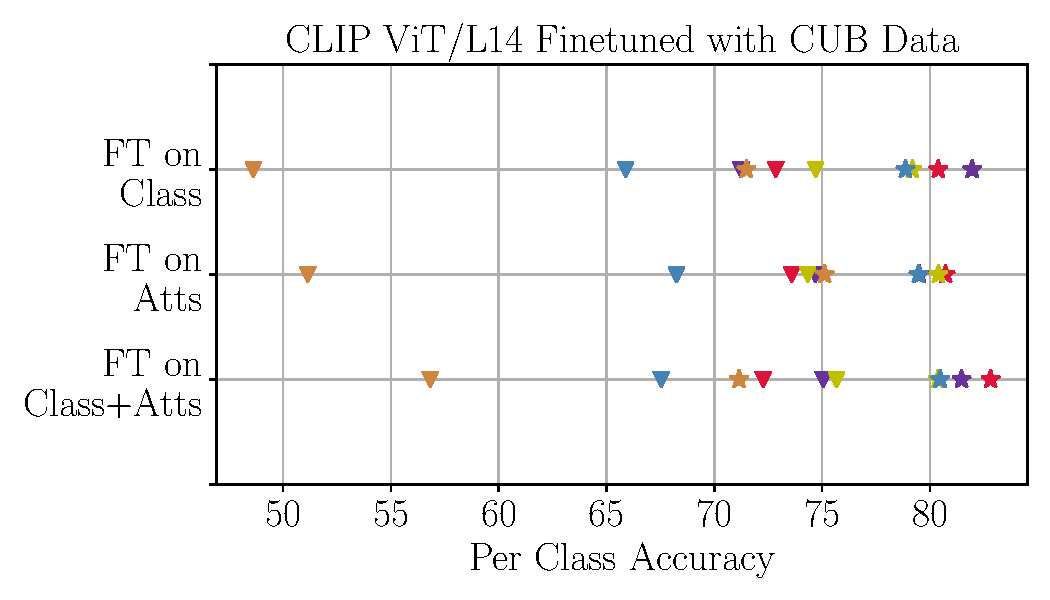
\includegraphics[width=.3\textwidth]{Images/gzsl_results_w_clip_finetuned_cub.pdf}\hfill
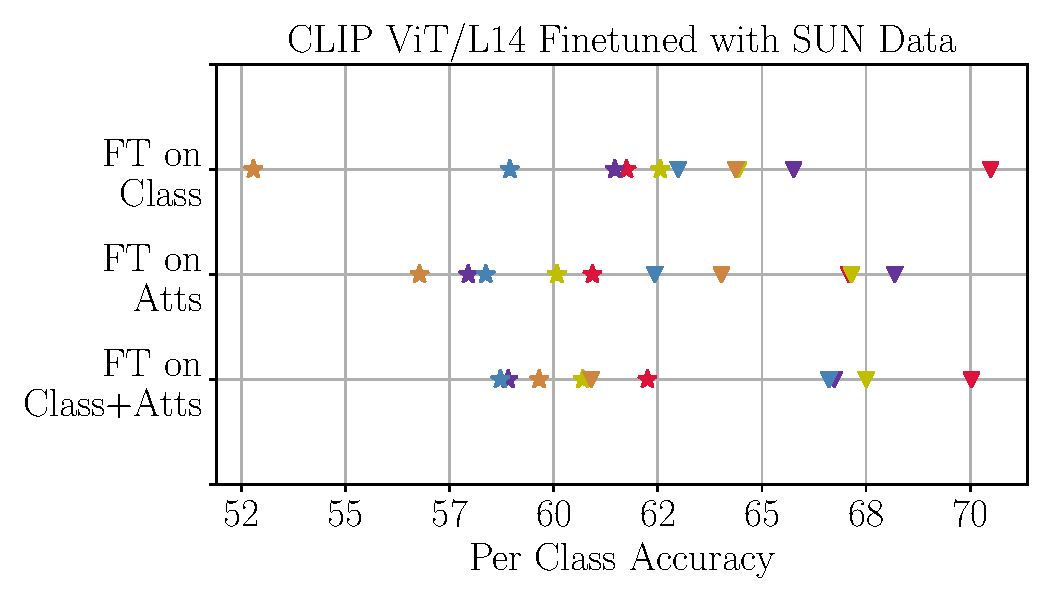
\includegraphics[width=.3\textwidth]{Images/gzsl_results_w_clip_finetuned_sun.pdf}\hfill
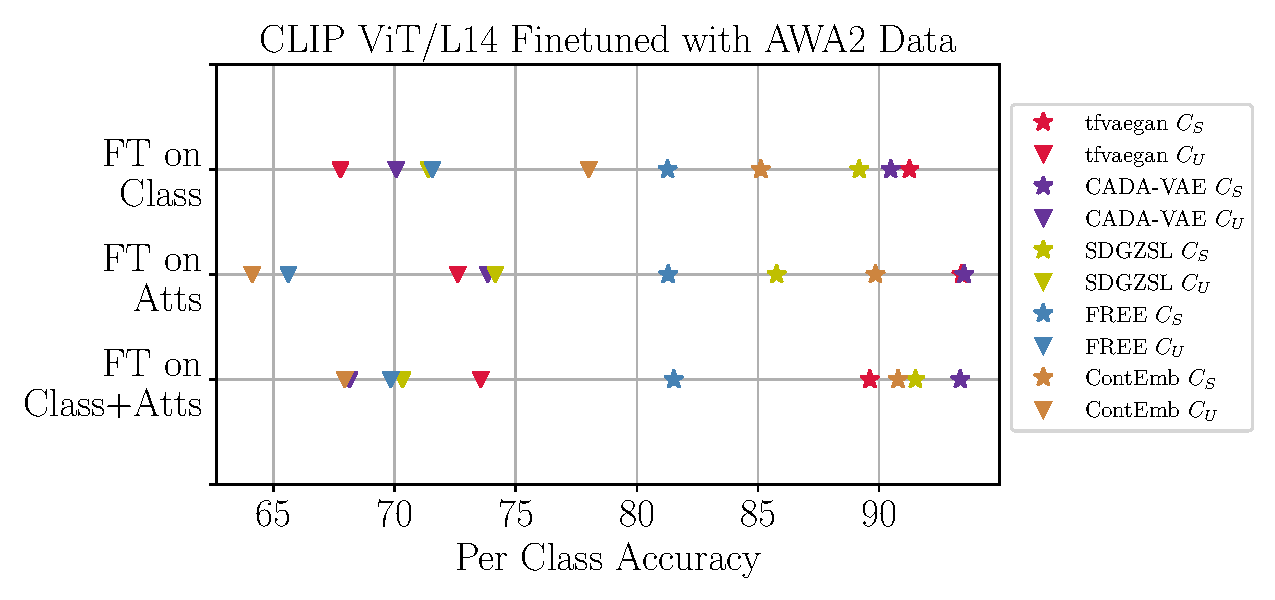
\includegraphics[width=.37\textwidth]{Images/gzsl_results_w_clip_finetuned_awa2.pdf}
\caption{Results when using features fine-tuned using the training seen classes with different GSZL methods. Overall, the generative-based methods (i.e., tfVAEGAN\cite{tfvaegan} and CADA-VAE\cite{CADA_VAE}) perform the best.}
\label{fig:finetuned_features_res}
\end{figure}




% \onecolumn

\section{Ethical Considerations}
\label{ethical}


Machine learning models still require collecting large amounts of annotated data. In the case of fine-grained recognition, these annotations often require specialized human knowledge. Zero-shot learning offers a way for bypassing the need to collect extensive amounts of data for training models for new classes of objects. 
We show that large-scale pre-trained models along with Generalized Zero-Shot Learning methods can obtain results that are competitive with the specialized knowledge from experts on classes that a trained model has never seen. We hope that the key insights and analysis provided in this paper will be useful in expanding and leveraging zero-shot research along with current progress in multi-modal learning. Allowing for the creation of models that do not depend on large amounts of data could be useful for practitioners without access to large scale resources or in domains where data is scarce such as the medical domain. 
